\chapter{Introduzione} %------------------------------ INTRODUZIONE
\thispagestyle{empty}
\newpage
\section{Scopo dello stage}
La tecnologia Text-To-Speech è molto diffusa al giorno d'oggi. In Italia però vi sono poche realtà esistenti che trattano questo campo. Una di esse è Mivoq S.r.l che è presente a Padova.\\
Mivoq si occupa di sintesi vocale, soprattutto dello sviluppo di engine Text-To-Speech (TTS) e della personalizzazione della voce.\\
Negli ultimi anni il lavoro di Mivoq si è focalizzato sullo sviluppo di due sistemi di sintesi vocale: uno è MaryTTS e l'altro è Speect.\\
Arrivati a un buon livello di maturazione dei due prodotti l'azienda ha deciso che era il momento di integrare i due engine TTS con un sistema operativo diverso da quello in cui erano stati sviluppati.\\
Il sistema operativo in questione era Microsoft Windows.\\
L'obiettivo dello stage era quindi far interagire i sistemi di sintesi vocale MaryTTS e Speect con il sistema operativo in questione tramite l'implementazione di una interfaccia SAPI~5.\\
Lo standard Speech Application Program Interface 5 (SAPI~5), sviluppato da Microsoft, permette di interfacciare il sistema operativo Microsoft Windows con un engine TTS tramite l'implementazione dei vari metodi messi a disposizione.
Il risultato finale che si vuole ottenere è la creazione di due moduli che permettano l'interazione tra gli engine utilizzati dall'azienda con il sistema operativo Windows tramite lo standard SAPI~5.\\
L'implementazione dovrà coprire la maggior parte delle funzionalità dagli engine TTS in relazione alle specifiche SAPI~5.

\section{Azienda Ospitante}
Mivoq S.r.l nata nel 2013, con sede a Padova si occupa di tecnologie vocali.\\
Il campo in cui è coinvolta maggiormente è il Text-To-Speech. Uno dei prodotti di maggior successo dell'azienda è la personalizzazione della voce, ovvero partendo da una voce reale è possibile creare una voce digitale molto simile al punto di partenza.\\
Questo è reso possibile dall'esperienza acquisita durante gli anni in ambito di ricerca e sviluppo nelle tecnologie vocali.
\begin{figure}[H]
\centering
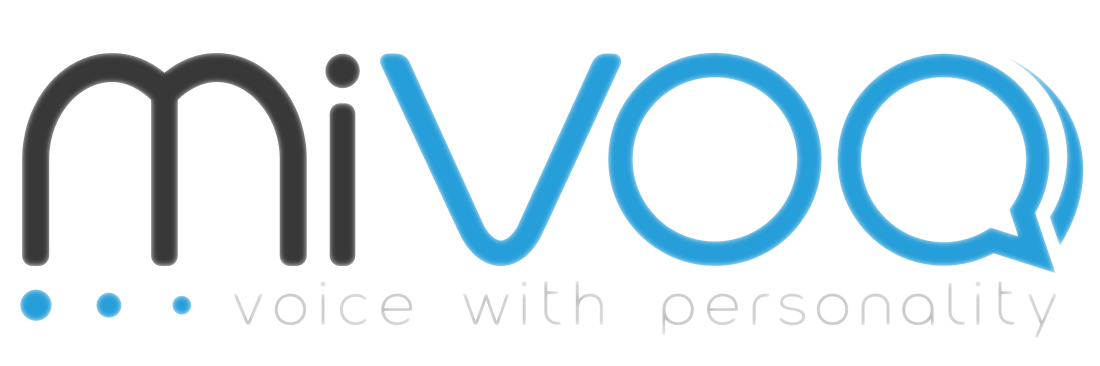
\includegraphics{images/logo-mivoq.png}
\caption{Logo di Mivoq S.r.l}
\end{figure}

\section{Struttura del documento}
 